Artificial Intelligence (AI) is an extremely broad field of research that is commonly summarized by the "Sense, Think, Act" cycle where an AI agent will first observe its surroundings, then think about the best response, and finally act. AI can be used in the form of Machine Learning (ML) and Deep Learning (DL) which are both subsets of AI. This hierarchy is illustrated in Figure \ref{fig:ai}. These two styles of ``teaching'' an AI agent (or model) are used to find patterns in data that are otherwise hard to recognize or, sometimes, unnoticeable to a human. ML and DL follow the same "Sense, Think, Act" cycle, but typically the Sense stage is more often referred to as the model learning information about the data. Thinking and Acting are typically combined into one stage for the model to make predictions about unknown data points.

\begin{figure}[!htb]
\centering
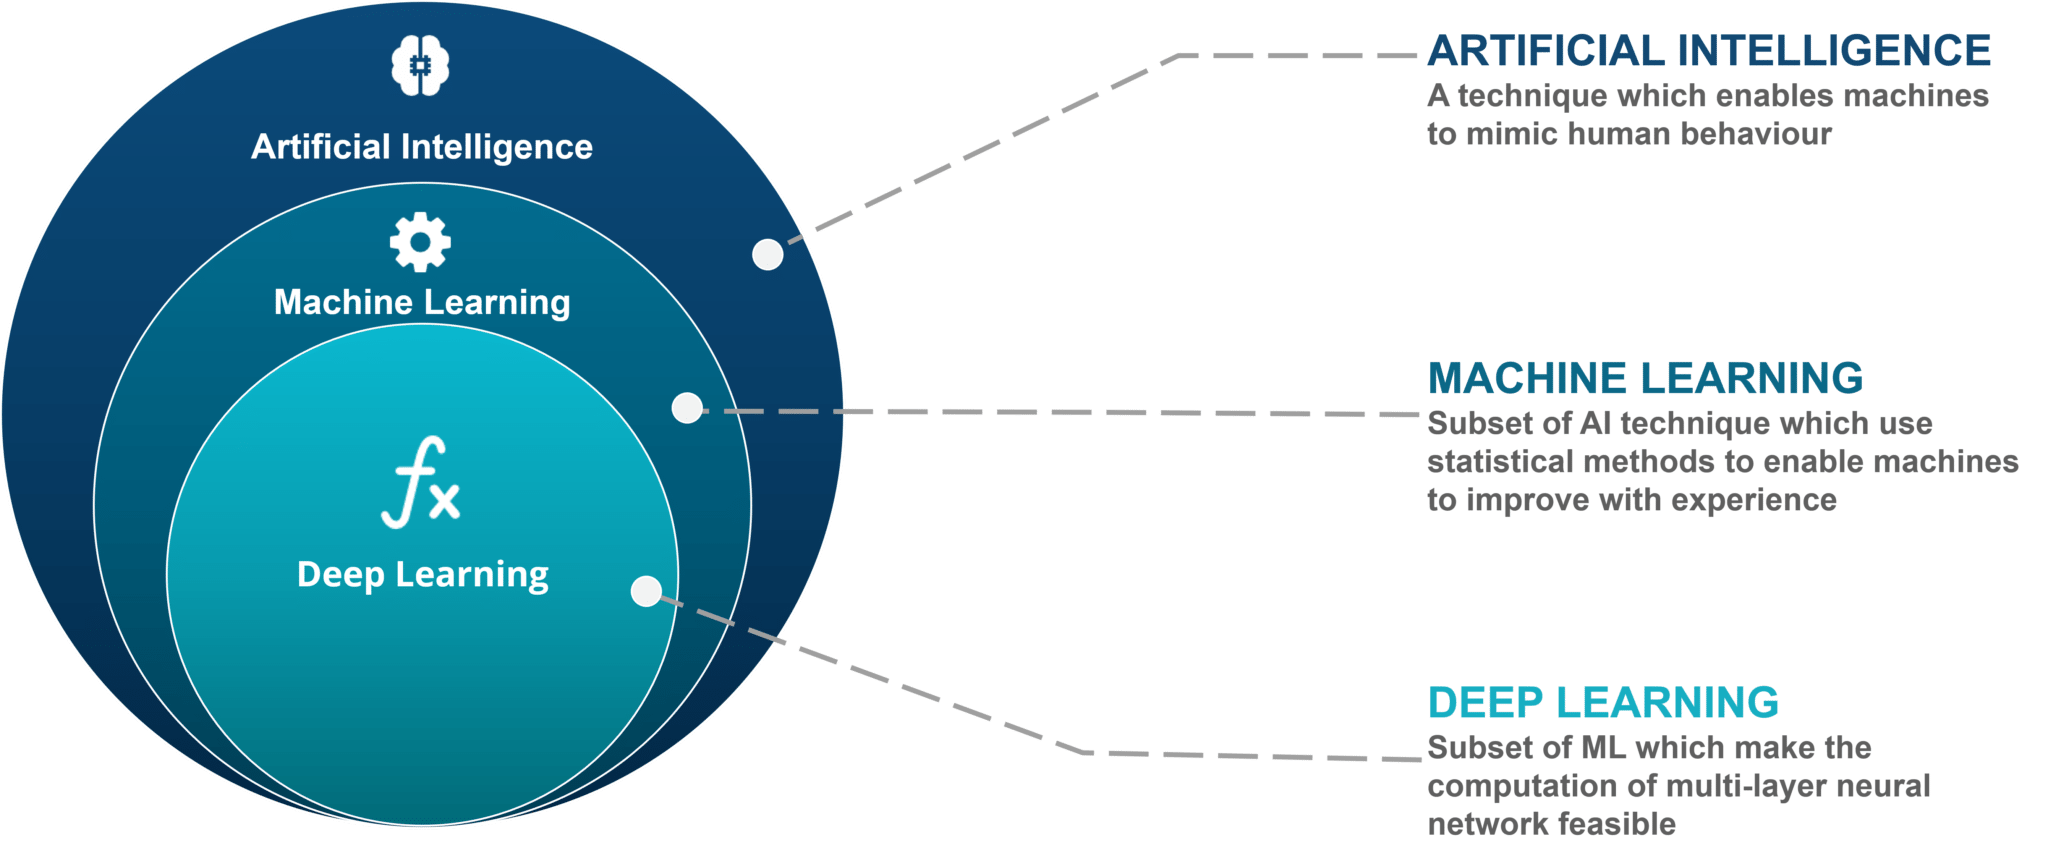
\includegraphics[width=.5\textwidth]{figures/AI-vs-ML-vs-Deep-Learning.png}
\caption{\label{fig:ai} AI vs ML vs DL - What's the Difference? \cite{atul_ai_2018}}
\end{figure}

In order for a machine to learn patterns in the data, a lot of data is required. This data typically contains multiple individual measurable properties or characteristics about what we are trying to model; these are called features. For example, if we were attempting to model house prices the list of features could include number of bedrooms, house size, lot size, etc. In addition to features, we have data about what we are trying to predict; this is typically called the response, but is sometimes also referred to as the label or class if the response is categorical. For our house model example, the price of the house would be the response. Using previous information about houses and their prices, we can train an ML model to find patterns in the data to be able to make accurate predictions on house prices for future homes that we have the features for but without the price.

This small example may seem simple, but as the complexity of the data grows, so does the complexity of the model. Currently in our example, the data collected is solely information about houses which only represents one channel of information, known as a modality, of what might be affecting house prices. Our model that uses house specifications to predict house price would be considered a unimodal model. If house prices were also affected by the weather, interactions with the realtor, etc., predicting house prices would need to consider all of these different modalities with a multimodal model.

As complexity of data inputs increase, DL models might be able to more accurately understand patterns from the features compared to ML models. In order to visualize what a DL model is doing, you can picture a person trying to uncrumple a paper ball. The crumpled paper ball is the complex input data and each small unfold of the paper ball is similar to a portion of the DL model working to understand a pattern in the data \cite{chollet-2021}. This technique might not be required for our house price prediction model because the problem space and type of input data is relatively simple.   
